%%% MORITZ 10' %%%

\section{Spinpräzession}
\subsection{Grundlagen}
\begin{frame}
\frametitle{Grundlagen: Spinpräzession}
  
\end{frame}

\subsection{Aufbau}
\begin{frame}
\frametitle{Aufbau: Spinpräzession}

\setbeamerfont{myfont}{size*=80}
\usebeamerfont{myfont}
\begin{figure}
    \centering
    \def\svgwidth{\textwidth}
    \input{../img/aufbauspinpraez.pdf_tex}
    \caption{Aufbau zur Messung der Spinpräzession.}
\end{figure}
\usebeamerfont{standard}

\begin{itemize}
  \item \textbf{Spule 1:} Kompensation von horizontalem Erdmagnetfeld
  \item \textbf{Spule 4:} Kompensation von vertikalem Erdmagnetfeld
  \item \textbf{Spule 5:} Ein- und Ausschalten von Magnetfeld mit 50\,Hz
\end{itemize}

\end{frame}

\subsection{Auswertung}

\begin{frame}
\frametitle{Auswertung: Spinpräzession}

\begin{figure}
    \centering
    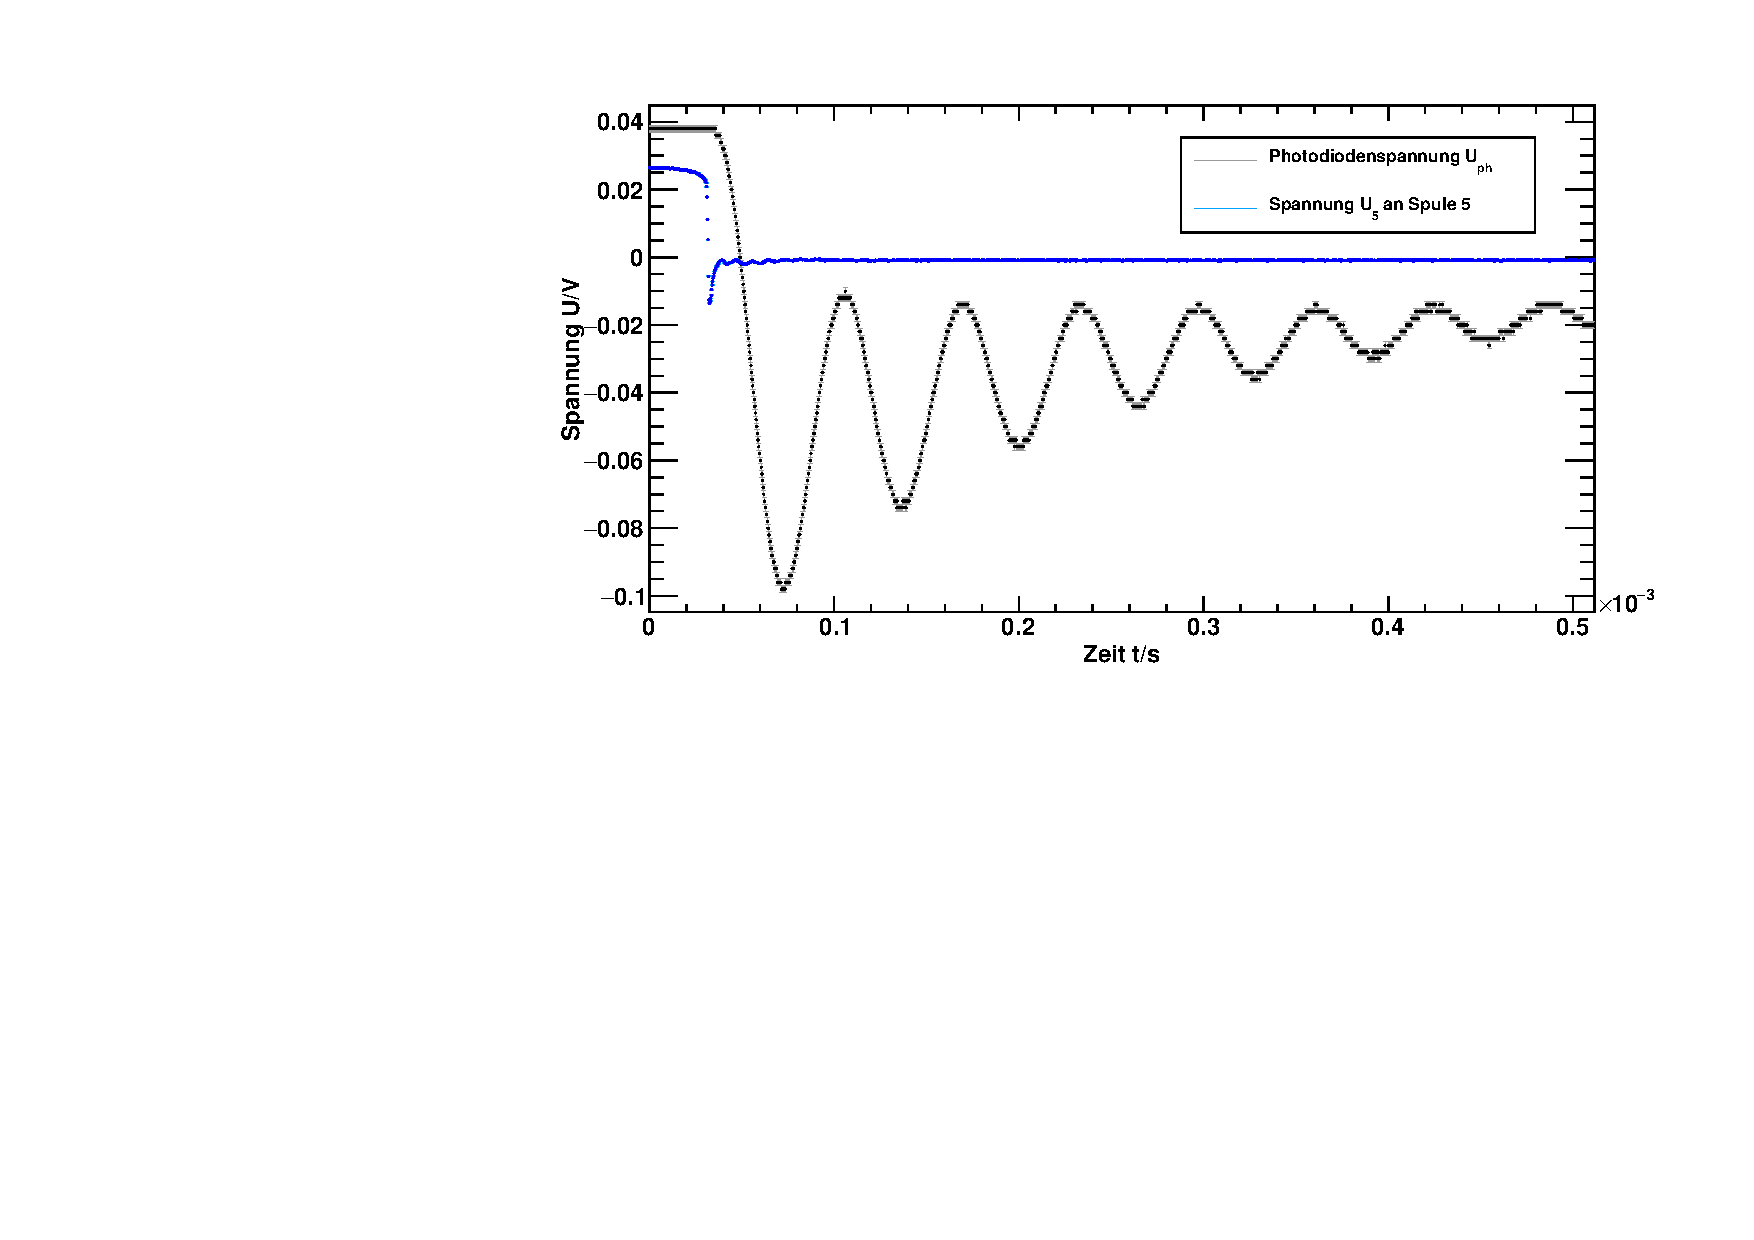
\includegraphics[width=\textwidth]{../img/02-63-7mA-087mA.pdf}
    \caption{Spinpräzession im schwachen Magnetfeld.}  
\end{figure} 
  
\end{frame}


\begin{frame}
\frametitle{Auswertung: Spinpräzession}

\begin{figure}
    \centering
    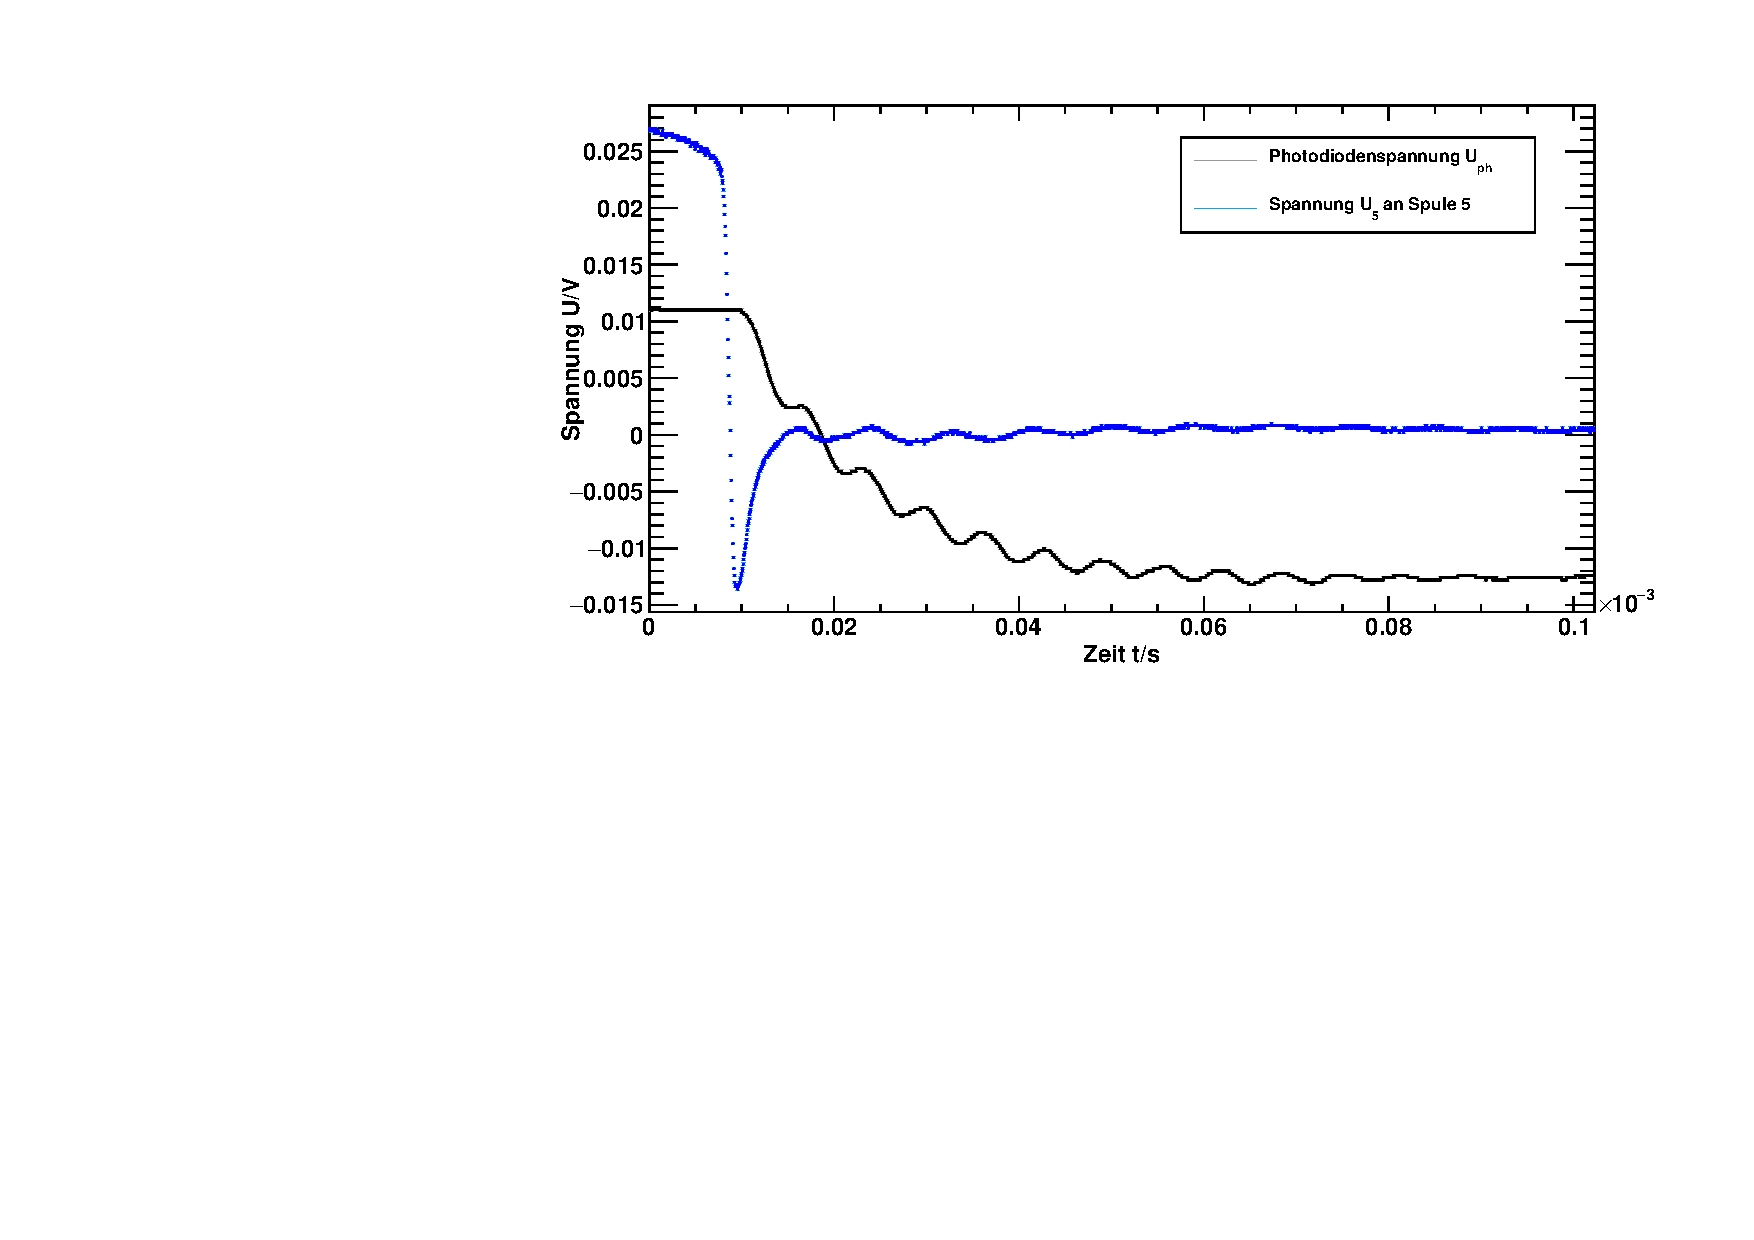
\includegraphics[width=\textwidth]{../img/02-63-7mA-020mA.pdf}
    \caption{Spinpräzession im starken Magnetfeld.}  
\end{figure} 
  
\end{frame}



\begin{frame}
\frametitle{Auswertung: Spinpräzession}

\begin{figure}
    \centering
    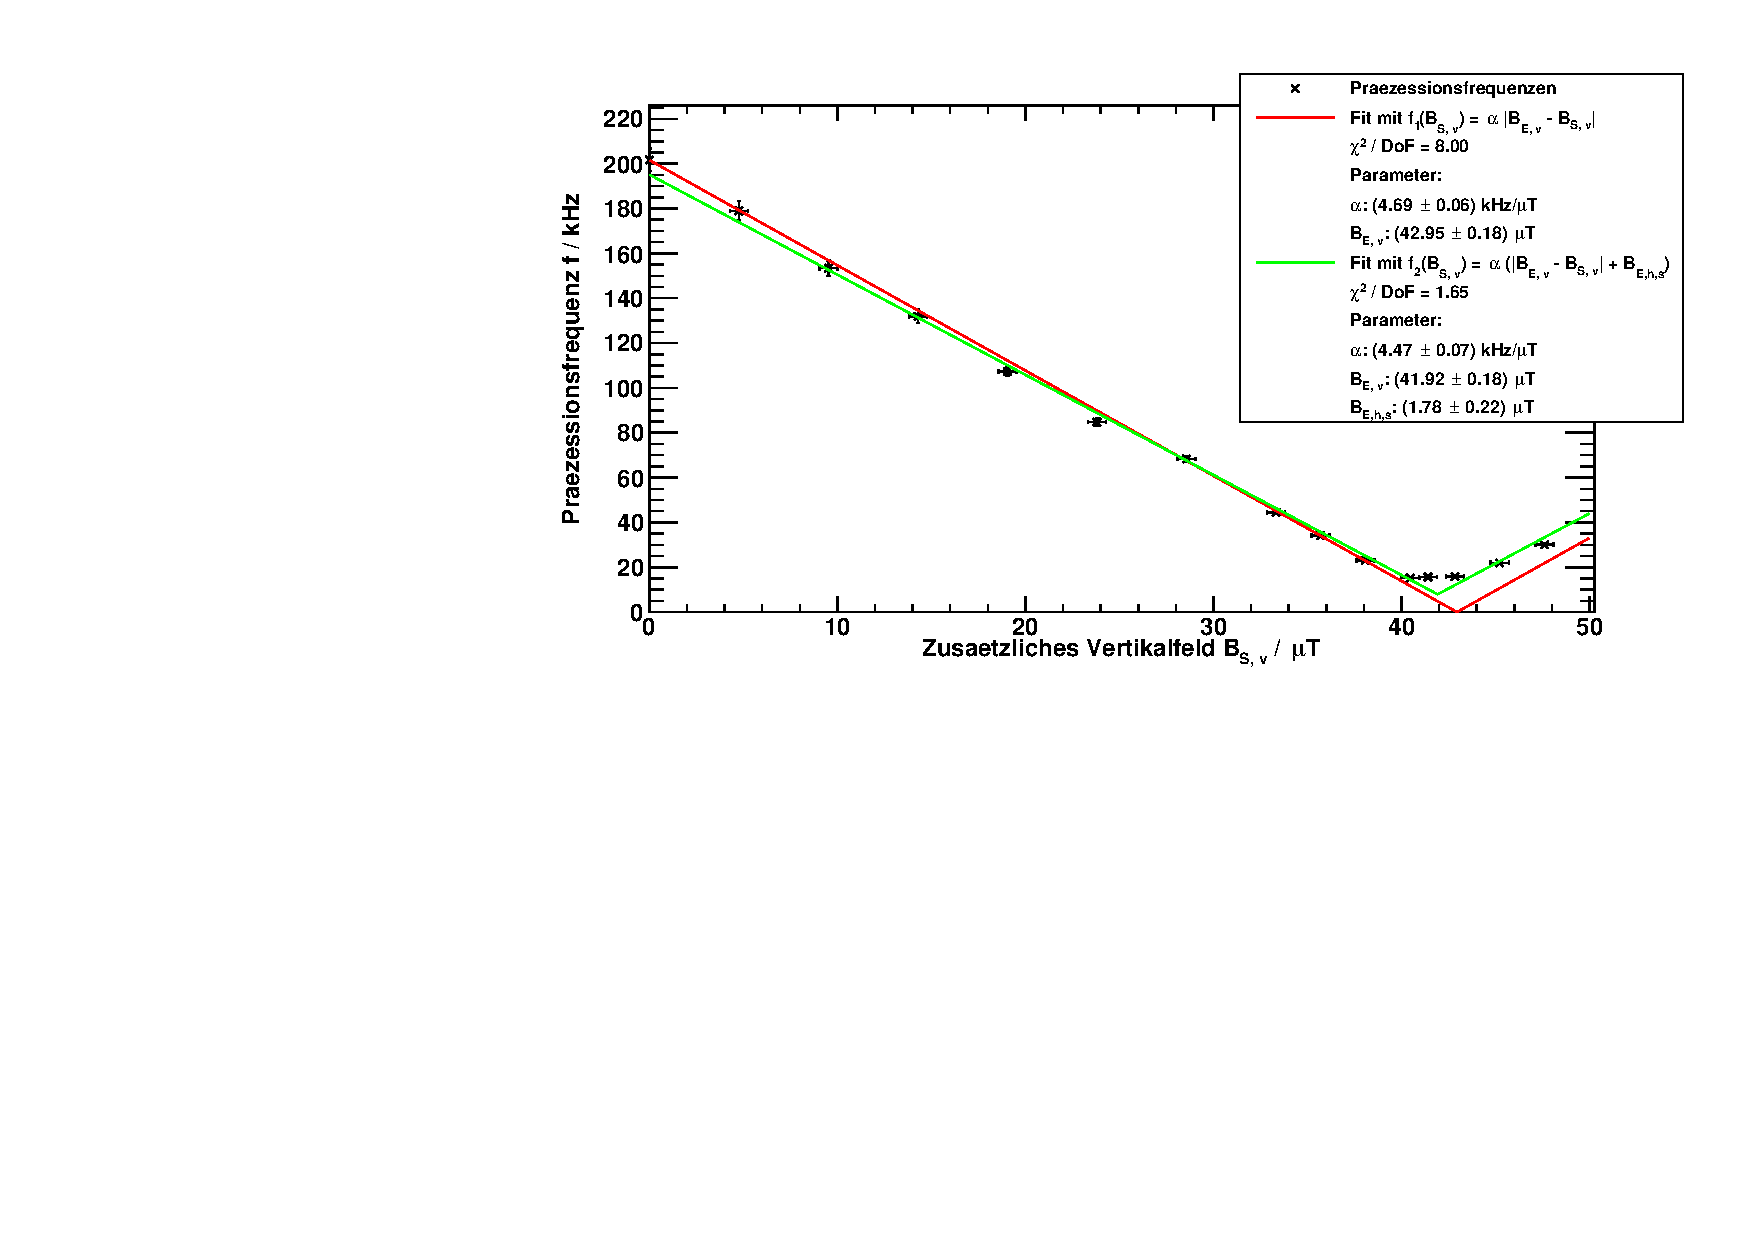
\includegraphics[width=\textwidth]{../img/Rb85.pdf}
    \caption{Magnetfeldabhängigkeit der Spinpräzessionsfrequenz.}  
\end{figure} 
  
\end{frame}


\begin{frame}
\frametitle{Auswertung: Spinpräzession}

Winkelberechnung
  
\end{frame}

\begin{frame}
\frametitle{Auswertung: Spinpräzession}

\begin{figure}
    \centering
    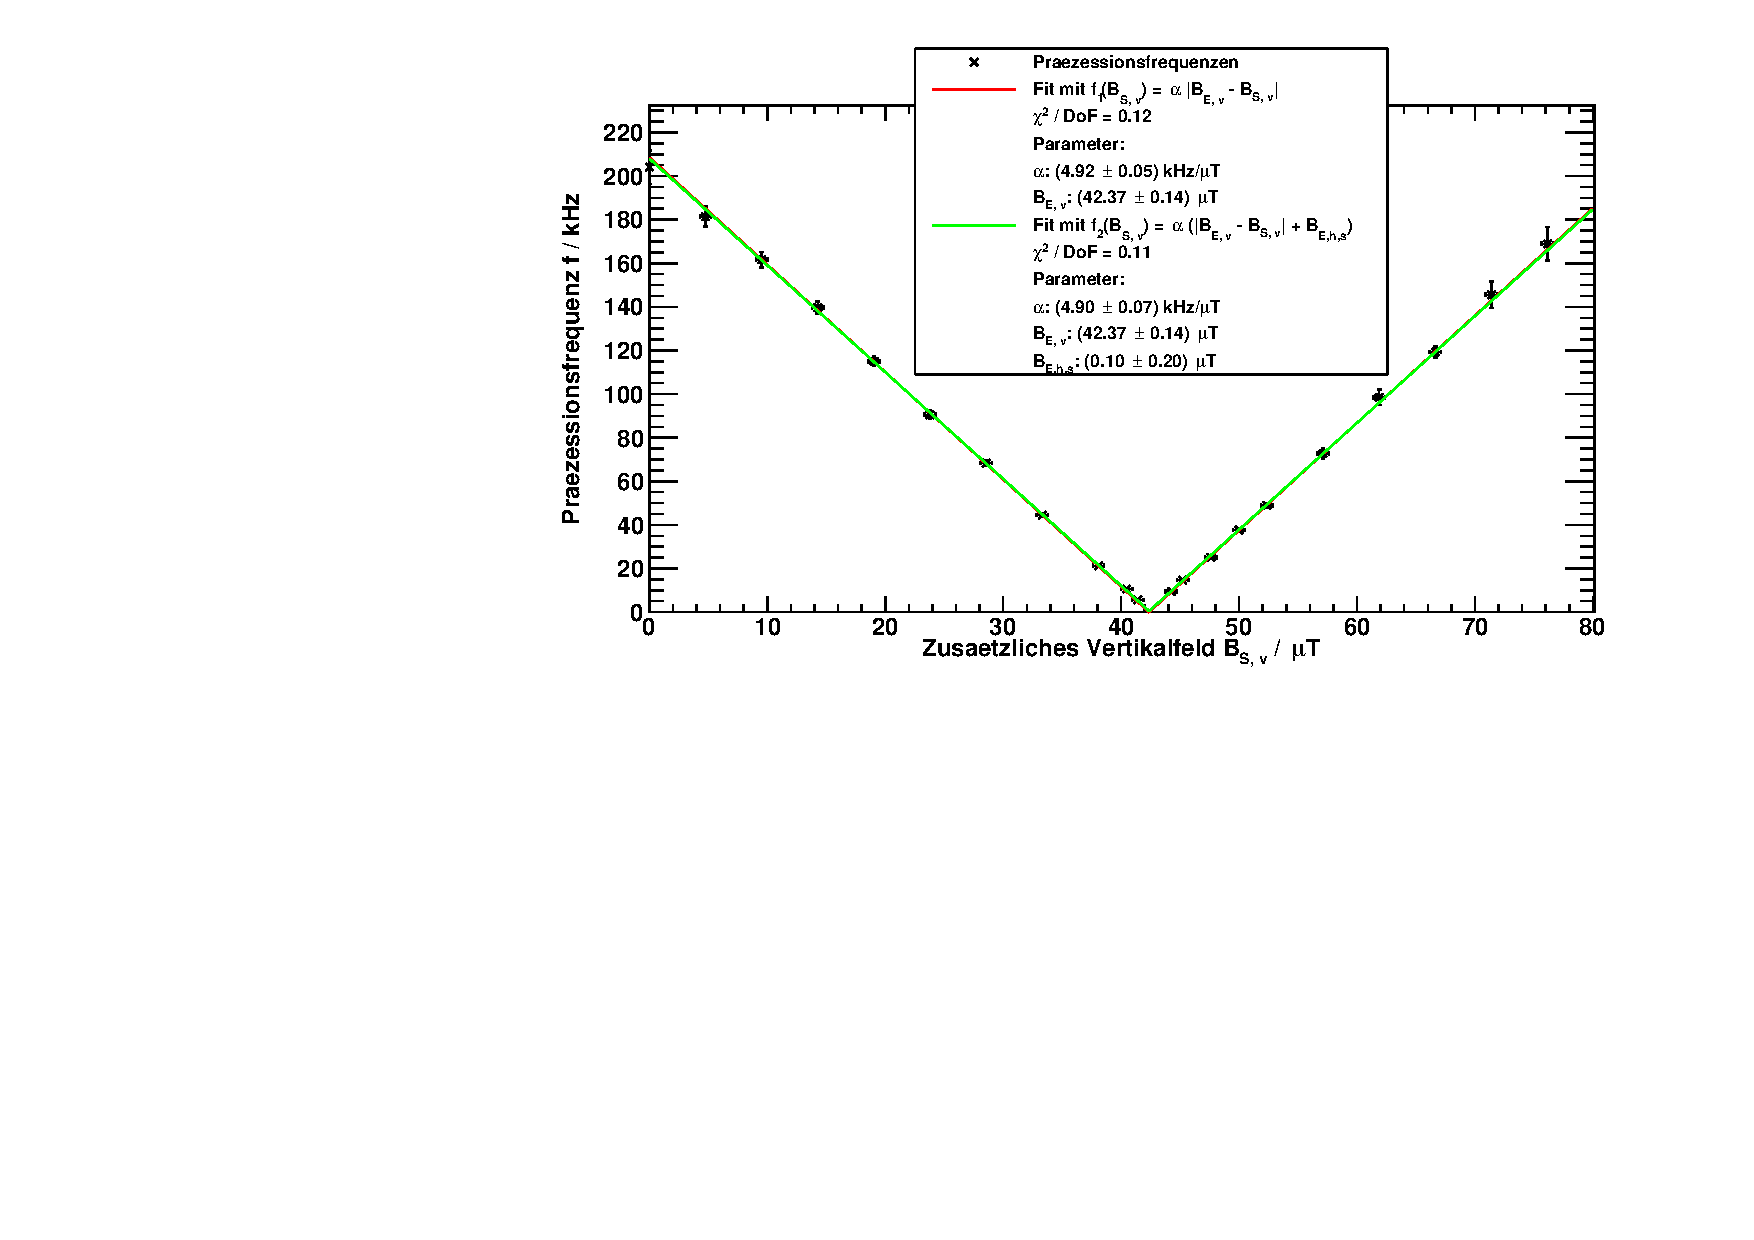
\includegraphics[width=\textwidth]{../img/Rb85_gedreht.pdf}
    \caption{Magnetfeldabhängigkeit der Spinpräzessionsfrequenz nach Ausrichtung des Versuchsaufbaus nach Norden.}  
\end{figure} 
  
\end{frame}




\begin{frame}
\frametitle{Auswertung: Spinpräzession}

\begin{figure}
    \centering
    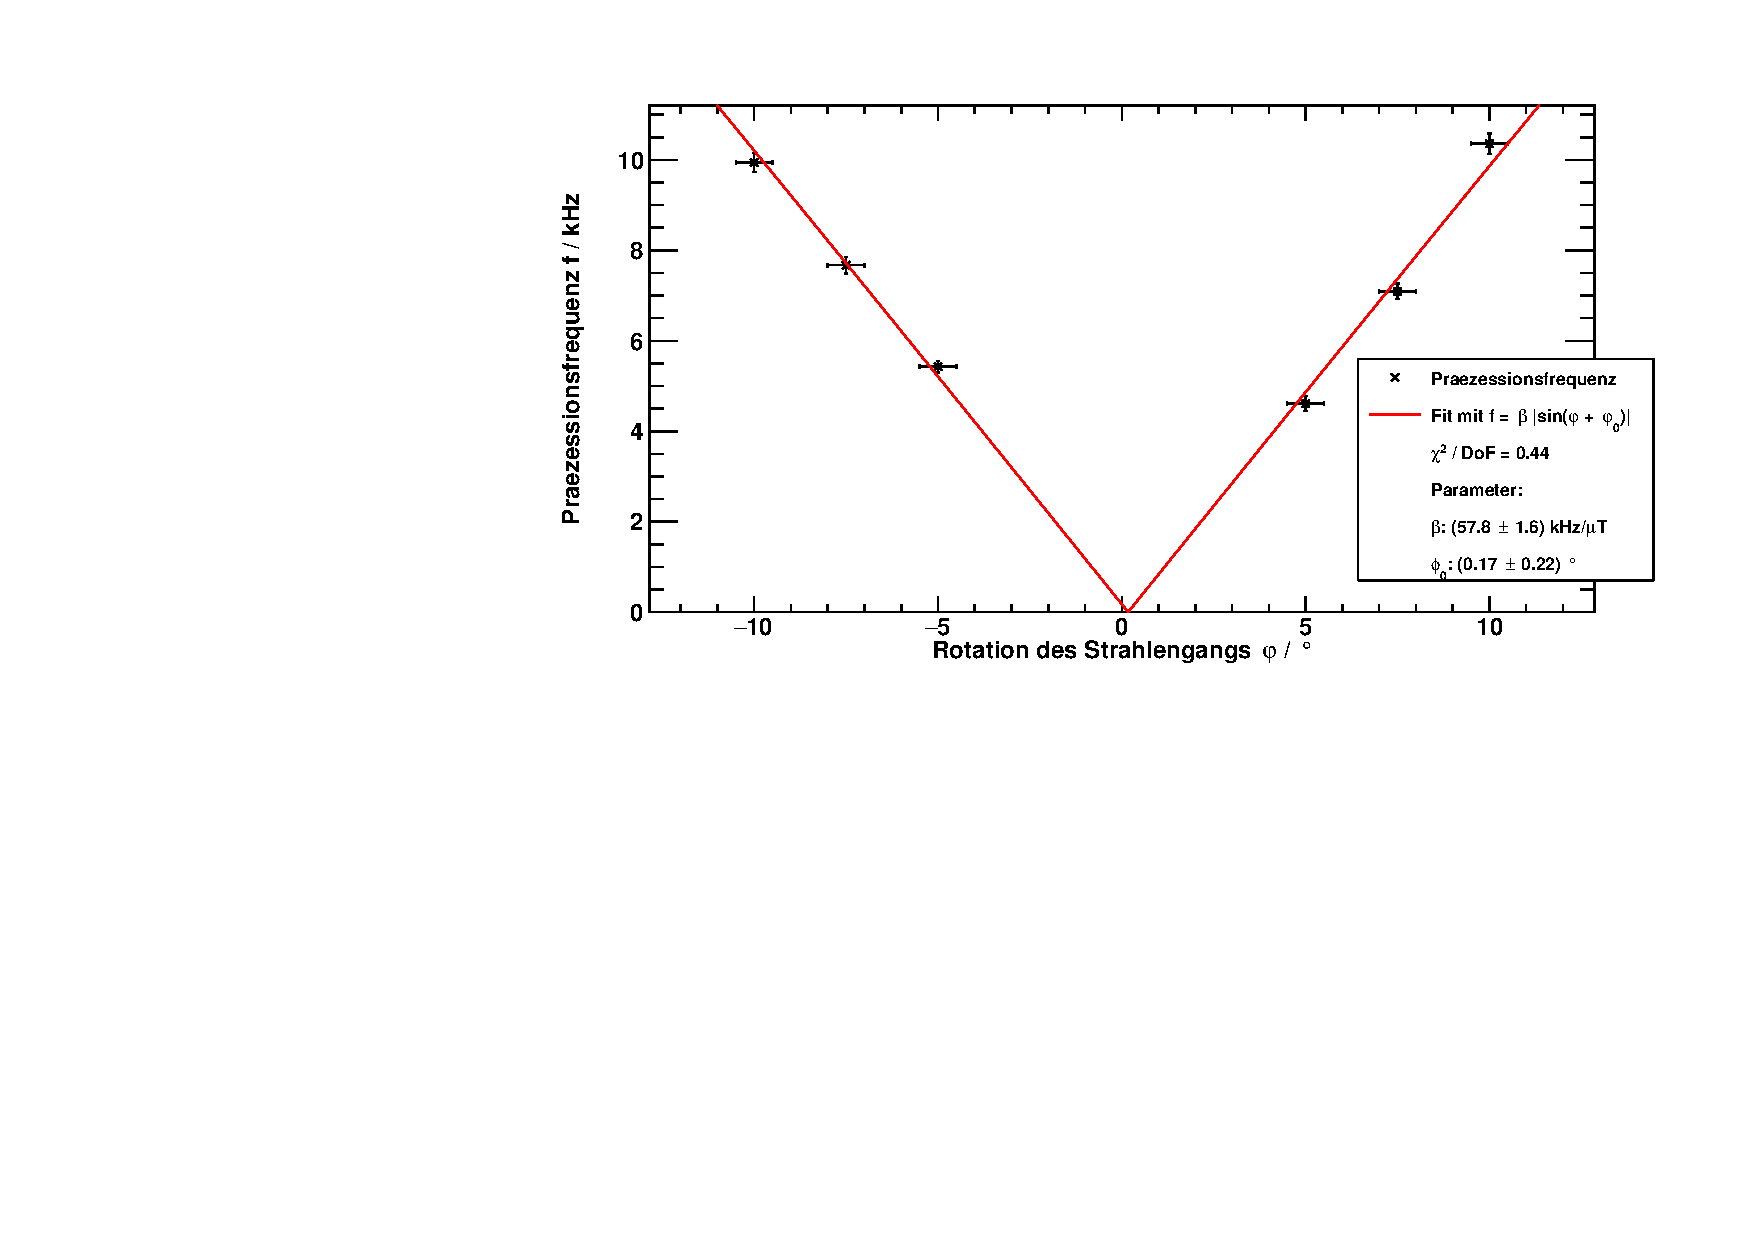
\includegraphics[width=\textwidth]{../img/winkel.pdf}
    \caption{Winkelabhängigkeit der Spinpräzessionsfrequenz.}  
\end{figure} 
  
\end{frame}
